\documentclass[11pt]{article}
\usepackage{amsmath,amsfonts,amssymb}
\usepackage{graphicx}
\usepackage{hyperref}
\usepackage{authblk}
\usepackage[backend=biber]{biblatex}
\newtheorem{lemma}{Lemma}
\newtheorem{definition}{Definition}
\newtheorem{remark}{Remark}

\addbibresource{../references.bib}
\title{The Abstract Universe: A Minimal Informational Model of Reality}
\author{Juha Meskanen}
\date{July 2025}

\begin{document}

\maketitle


\begin{abstract}
    Building on our earlier proposal that the universe is fundamentally informational in nature,
    we propose a radically minimalist foundation for physics based on information only.
    The framework assumes no primitive physical substrate—no predefined spacetime, particles, or fields.
    Everything we observe, from matter to consciousness, is modeled as an emergent structure within a fundamentally informational universe.
\end{abstract}

\section{A Minimal Informational Model of Reality}

This section describes a minimal model of reality based on the hypothesis that observers are substrings of bitstrings. No further structure is assumed.

\subsection{Ontological Basis}

We assume:

\begin{enumerate}
    \item Reality consists of binary strings of length $n$: $b \in \{0,1\}^n$.
    \item An observer is a subset of positions $P \subseteq \{0,1,\dots,n-1\}$.
    \item Observed reality is defined by selecting those positions: $O = b|_P$.
\end{enumerate}

No concept of time, matter, or causality is assumed beyond this.

\subsection{Subjective Time as Emergent Ordering}

The observer’s subjective time emerges from the intrinsic ordering of its bit-selector subset. Specifically, each observer defines a sequence
\[
    P = (i_0, i_1, \dots, i_k),
\]
where \(i_j \in \{0,\dots,n-1\}\). This sequence imposes a \emph{structural} temporal axis—an emergent phenomenon based entirely on the ordering of positions—without invoking any active or external process.

\subsection{Formal Definition of Observer Memory via Structural Similarity}

Let \(U = (b_0,b_1,\dots,b_{N-1})\). An observer is defined by a subset \(P\subseteq \{0,\dots,N-1\}\) and derives bits \(O = U|_P\).

We introduce \emph{memory} as follows:

\begin{definition}[Memory via Similarity]
    An observer exhibits memory if there exist non-empty subsets \(M\subseteq P\) and \(S\subseteq \{0,\dots,N-1\}\) such that
    \[
        \mathrm{Sim}(U|_M, U|_S)\;\ge\;\theta,
    \]
    for a threshold \(\theta\in[0,1]\).
\end{definition}

Here, \(\mathrm{Sim}\) is a similarity function. For equal-length bitstrings:
\[
    \mathrm{Sim}(x,y)=1-\frac1{|x|}\sum_{j=1}^{|x|} |x_j-y_j|.
\]
If \(x,y\) differ in length, interpretations include truncating or extending the shorter string with a neutral value.

\subsection{Probability and Observer Prevalence}

We define probability as a relative frequency over compatible observers:

\begin{definition}[Observer Probability]
    Let $S$ be the set of all observers compatible with universe $U$. Then the probability of $O$ is
    \[
        \mathbb{P}(O) = \frac{|\{O' \in S : O' \sim O\}|}{|S|},
    \]
    where $\sim$ denotes structural similarity above a fixed threshold.
\end{definition}

\subsection{Observer Continuity Lemma (OCL)}

Let \(O=(o_1,\dots,o_n)\) be an observer’s internal trajectory and \(F=(f_1,\dots,f_n)\) be corresponding universe-frame bitstrings. We require:

\[
    \exists\;\epsilon>0\;\text{such that}\;\mathrm{Sim}(o_i, f_i)\ge\epsilon\;\text{for all }i.
\]

This condition ensures structural continuity and provides the formal basis for “memory” and coherent subjective experience without appealing to causal interactions.

\subsection{Observer-Centric Universe Compression Principle (OCUCP)}

We propose the following principle:

\begin{quote}
    The most probable universes are those that maximize the number of compatible observer trajectories under structural continuity constraints.
\end{quote}

Formally, let $U$ be a candidate universe, and $T(U)$ the set of observer trajectories satisfying the OCL. Then:

\[
    \mathbb{P}(U) \propto |T(U)|.
\]

This leads to a selection bias toward simple, compressible universes with many observers.

\subsection{Compression and the Wavefunction}

\begin{definition}[Compression Bias Principle (CBP)]
    Let \(F\) be a sequence of universe frames. Let \(C(F)\) denote its compressed bit-length. Then:
    \[
        \#\{\text{observer trajectories embedded in }F\}\;\propto\; \frac{1}{C(F)}.
    \]
\end{definition}

From this emerges a model of the quantum-like wavefunction:

\begin{itemize}
    \item The observer’s internal model maintains past states \(\{o_1,\dots,o_t\}\).
    \item Potential future continuations \(\{o_{t+1},\dots,o_{t+k}\}\) are extrapolated via compressive pattern completion.
    \item If the compression basis is Fourier/sinusoidal, the predicted frames are inherently smooth and oscillatory.
    \item Multiple continuations form a \emph{superposition}, weighted by compressibility, with interference patterns arising from shared substructures.
\end{itemize}

Under this interpretation, the wavefunction is not a physical field but a \textbf{computationally optimal compression model} used by the observer.

\subsection{Entanglement and Memory Sharing}

Let two observers \(O_1, O_2\) share a common prefix \(S\). Then:

\begin{definition}[Entangled Observers]
    Observers \(O_1\) and \(O_2\) are entangled if \(\mathrm{Sim}(O_1|_S, O_2|_S)\ge\theta\) for some threshold \(\theta\).
\end{definition}

Such observers exhibit correlated outcomes without communication, due to shared structural ancestry.


\section{Discussion and Implications}

\subsection{Finite Information}

We do \emph{not assume} that reality must be finite in absolute terms. Instead, finiteness follows from two operational principles:
\begin{enumerate}
    \item Conservation of information implies bounded total informational content.
    \item An observer can \emph{only} access and encode a finite subset of information.
\end{enumerate}
Infinite structures remain mathematically conceivable but play no role in the observer’s emergent perception.

\subsection{Wavefunction as Compression Algorithm}

We argue the quantum wavefunction arises from the \textbf{most efficient compression scheme} a finite observer can construct. Periodic functions—especially sine waves—are favored due to their optimal information density and simplicity, consistent with empirical smoothness in physical laws.

\subsection{Ontological Neutrality}

This model does not presuppose the existence of a physical substrate. Bitstrings may be realized physically, virtually, or abstractly. The theory is agnostic to ontology beyond information and observer-defined structure.

\subsection{Empirical Implications}

While abstract, this framework generates testable implications:

\begin{itemize}
    \item The universe should exhibit compressible, recursive structure.
    \item High-entropy or uncorrelated states (e.g. pure noise) should rarely support coherent observers.
    \item Apparent laws of physics reflect compressibility bias, not ontological necessity.
\end{itemize}



\section{Supplementary Material: Simulation}

We present a simulation program implementing the formal model as a Python script.

This simulation models an observer embedded in a spacetime constructed from finite information. It uses a compressed representation of the universe via Fourier basis functions and identifies regions where an observer pattern is likely to occur. The simulation is grounded in the principles of informational physics and is designed to reflect quantum-like probability distributions from a discrete, observer-centric perspective.

\subsection*{2.1. Spacetime Representation}

Spacetime is represented as a 2D discrete binary matrix $S \in \{0, 1\}^{H \times W}$, where:
\begin{itemize}
    \item $W$: width (spatial extent) of the universe,
    \item $H$: height (temporal extent),
    \item Each entry $S_{i,j} = 1$ or $0$ indicates the presence or absence of a bit at spacetime coordinate $(i,j)$.
\end{itemize}

This binary field $S$ is derived from a real-valued wavefield $R \in \mathbb{R}^{H \times W}$, constructed as:
\begin{equation}
    R = \mathcal{F}^{-1}(F),
\end{equation}
where $F$ is a sparse complex-valued matrix of Fourier coefficients populated with $n_f$ random components, and $\mathcal{F}^{-1}$ denotes the 2D inverse Fourier transform (IFFT). The binary field $S$ is obtained by thresholding $R$:
\begin{equation}
    S_{i,j} =
    \begin{cases}
        1 & \text{if } R_{i,j} > \theta, \\
        0 & \text{otherwise},
    \end{cases}
\end{equation}
where $\theta$ is a threshold parameter (typically $\theta = 0$).

\subsection*{2.2. Observer Representation}

The observer is modeled as a binary pattern $O \in \{0,1\}^{k \times k}$, where $k$ is the observer's spatiotemporal extent. A typical example is a disk-like structure, implying emergence, growth, and fading phases in spacetime.

\subsection*{2.3. Match Score}

To identify where the observer is likely to occur in the spacetime field, a convolution operation is applied:
\begin{equation}
    C = S \ast O,
\end{equation}
where $\ast$ denotes 2D cross-correlation (equivalent to convolution with a flipped kernel). The total match count is computed as:
\begin{equation}
    \text{Matches} = \sum_{i,j} \delta(C_{i,j}, \sum O),
\end{equation}
where $\delta(a,b)$ is the Kronecker delta, equal to $1$ if $a = b$, and $0$ otherwise.

\subsection*{2.4. Probability Map}

The continuous wavefield $R$ is convolved with the observer pattern $O$ to construct a real-valued overlap map:
\begin{equation}
    \Psi(i,j) = (R \ast O)_{i,j},
\end{equation}
and the squared amplitude of this overlap produces a normalized probability map:
\begin{equation}
    P(i,j) = \frac{|\Psi(i,j)|^2}{\max_{i,j} |\Psi(i,j)|^2},
\end{equation}
which gives the relative probability of the observer being instantiated at location $(i,j)$.

\subsection*{2.5. Top Matches}

From the map $P$, the top-$N$ local maxima are selected as the most likely observer instantiations:
\[
    \text{TopMatches} = \{(i,j) \in \text{argmax}_N P(i,j)\}
\]
with spatial masking applied to prevent overlapping detections.

\subsection*{3. Summary}

This simulation constructs a discrete spacetime as a binarized inverse Fourier field and embeds an observer as a localized binary pattern. The overlap of this pattern with the wavefield yields a probability distribution consistent with a quantum mechanical interpretation. The representation is fully informational, observer-centered, and compressive, with no external constants beyond simulation parameters.

Importantly, the simulation parameters should not be interpreted as predefined axioms of the theory. Ideally, the simulation would explore all possible observers across all possible universes and encodings. However, due to computational constraints, we focus here on a single observer and a single choice of parameters.

The program allows the observer to be defined as a 2D shape, where the $x$-axis corresponds to space and the $y$-axis to time.

\begin{figure}[ht]
    \centering
    \begin{minipage}{0.8\textwidth}
        \begin{verbatim}
    observer = [
        [0, 0, 1, 0, 0],
        [0, 1, 1, 1, 0],
        [1, 1, 1, 1, 1],
        [1, 1, 0, 1, 1],
        [1, 1, 1, 1, 1],
        [1, 1, 0, 1, 0],
        [1, 0, 1, 0, 1]]
  \end{verbatim}
    \end{minipage}
    \caption{One dimensional observer evolving in time. }
\end{figure}

This pattern is then converted into a wavefunction via Fourier transformation.

\begin{figure}[h!]
    \centering
    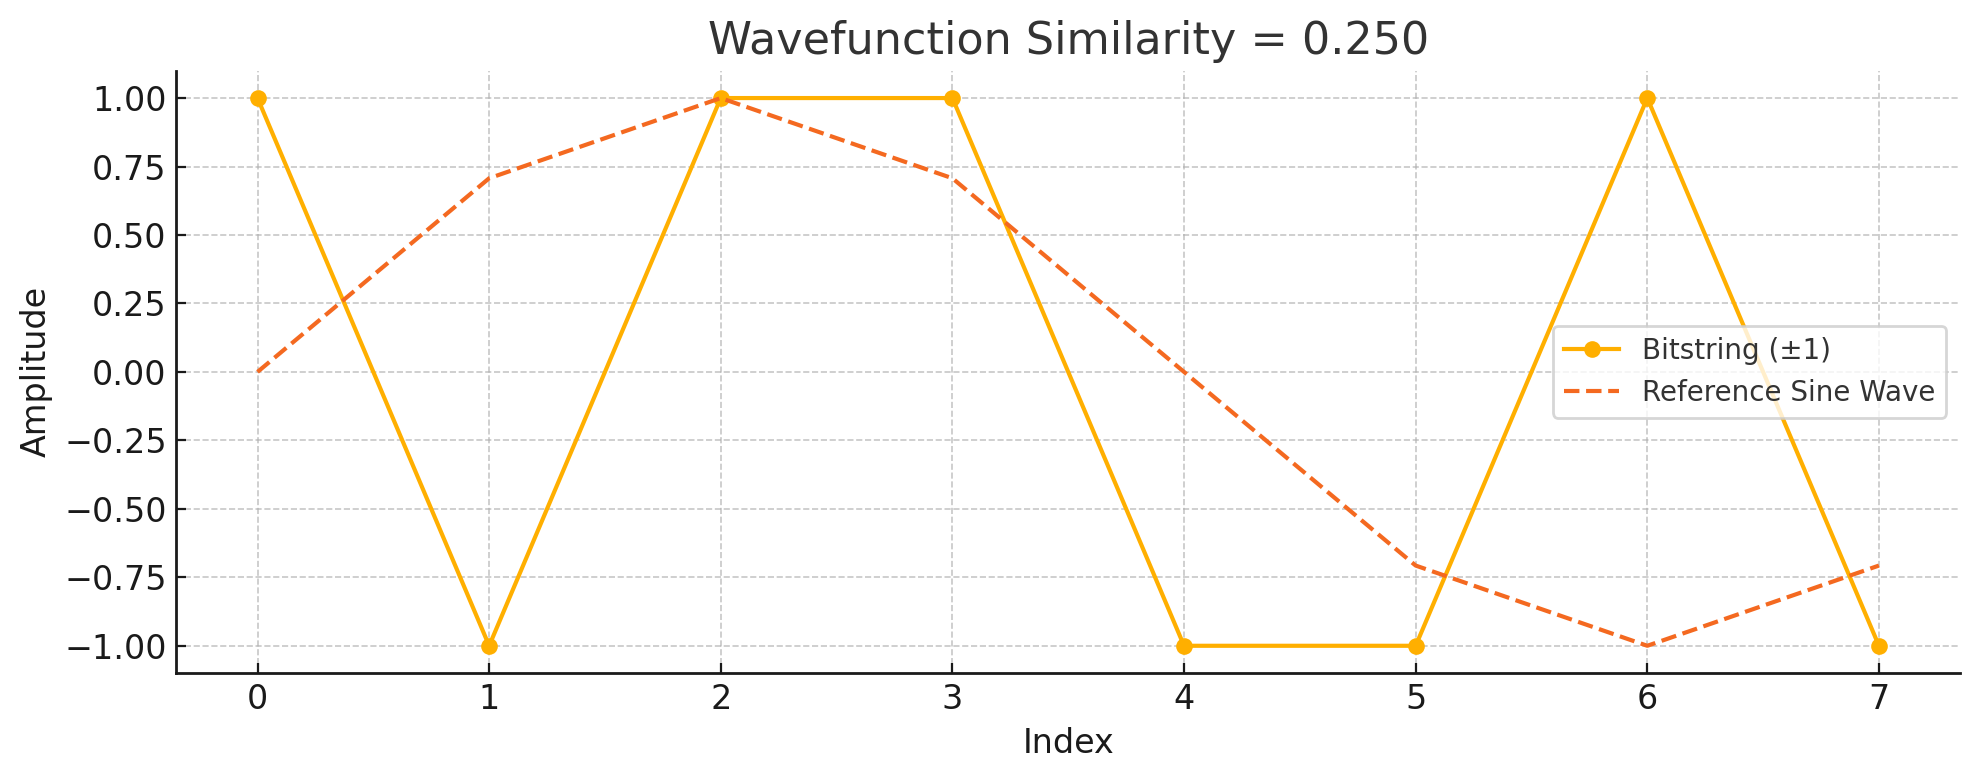
\includegraphics[width=1.0\textwidth]{figures/wavefunction_similarity.png}
    \caption{The wavefunction representation of the discrete observer.}
    \label{fig:wavefunction_similarity}
\end{figure}

A finite number of Fourier components is used for compression, naturally leading to a quantum-like interpretation of observer presence via wavefunction overlap.

\subsection{Output and Results}

The program generates four plots to visualize the universe that best supports the specified observer.

These demonstrate:
\begin{itemize}
    \item \textbf{Wavefunctions} as a natural consequence of compressible, high-structure bitstring universes.
    \item \textbf{Interference} as a mechanism for observer motif detection.
    \item \textbf{Physics} as emergent structure shaped by informational filtering—where only configurations consistent with compressible observers persist.
\end{itemize}

From this perspective, quantum behavior, continuity, and even time emerge as statistical artifacts of optimal observer embedding in compressible informational structures.

\begin{figure}[h!]
    \centering
    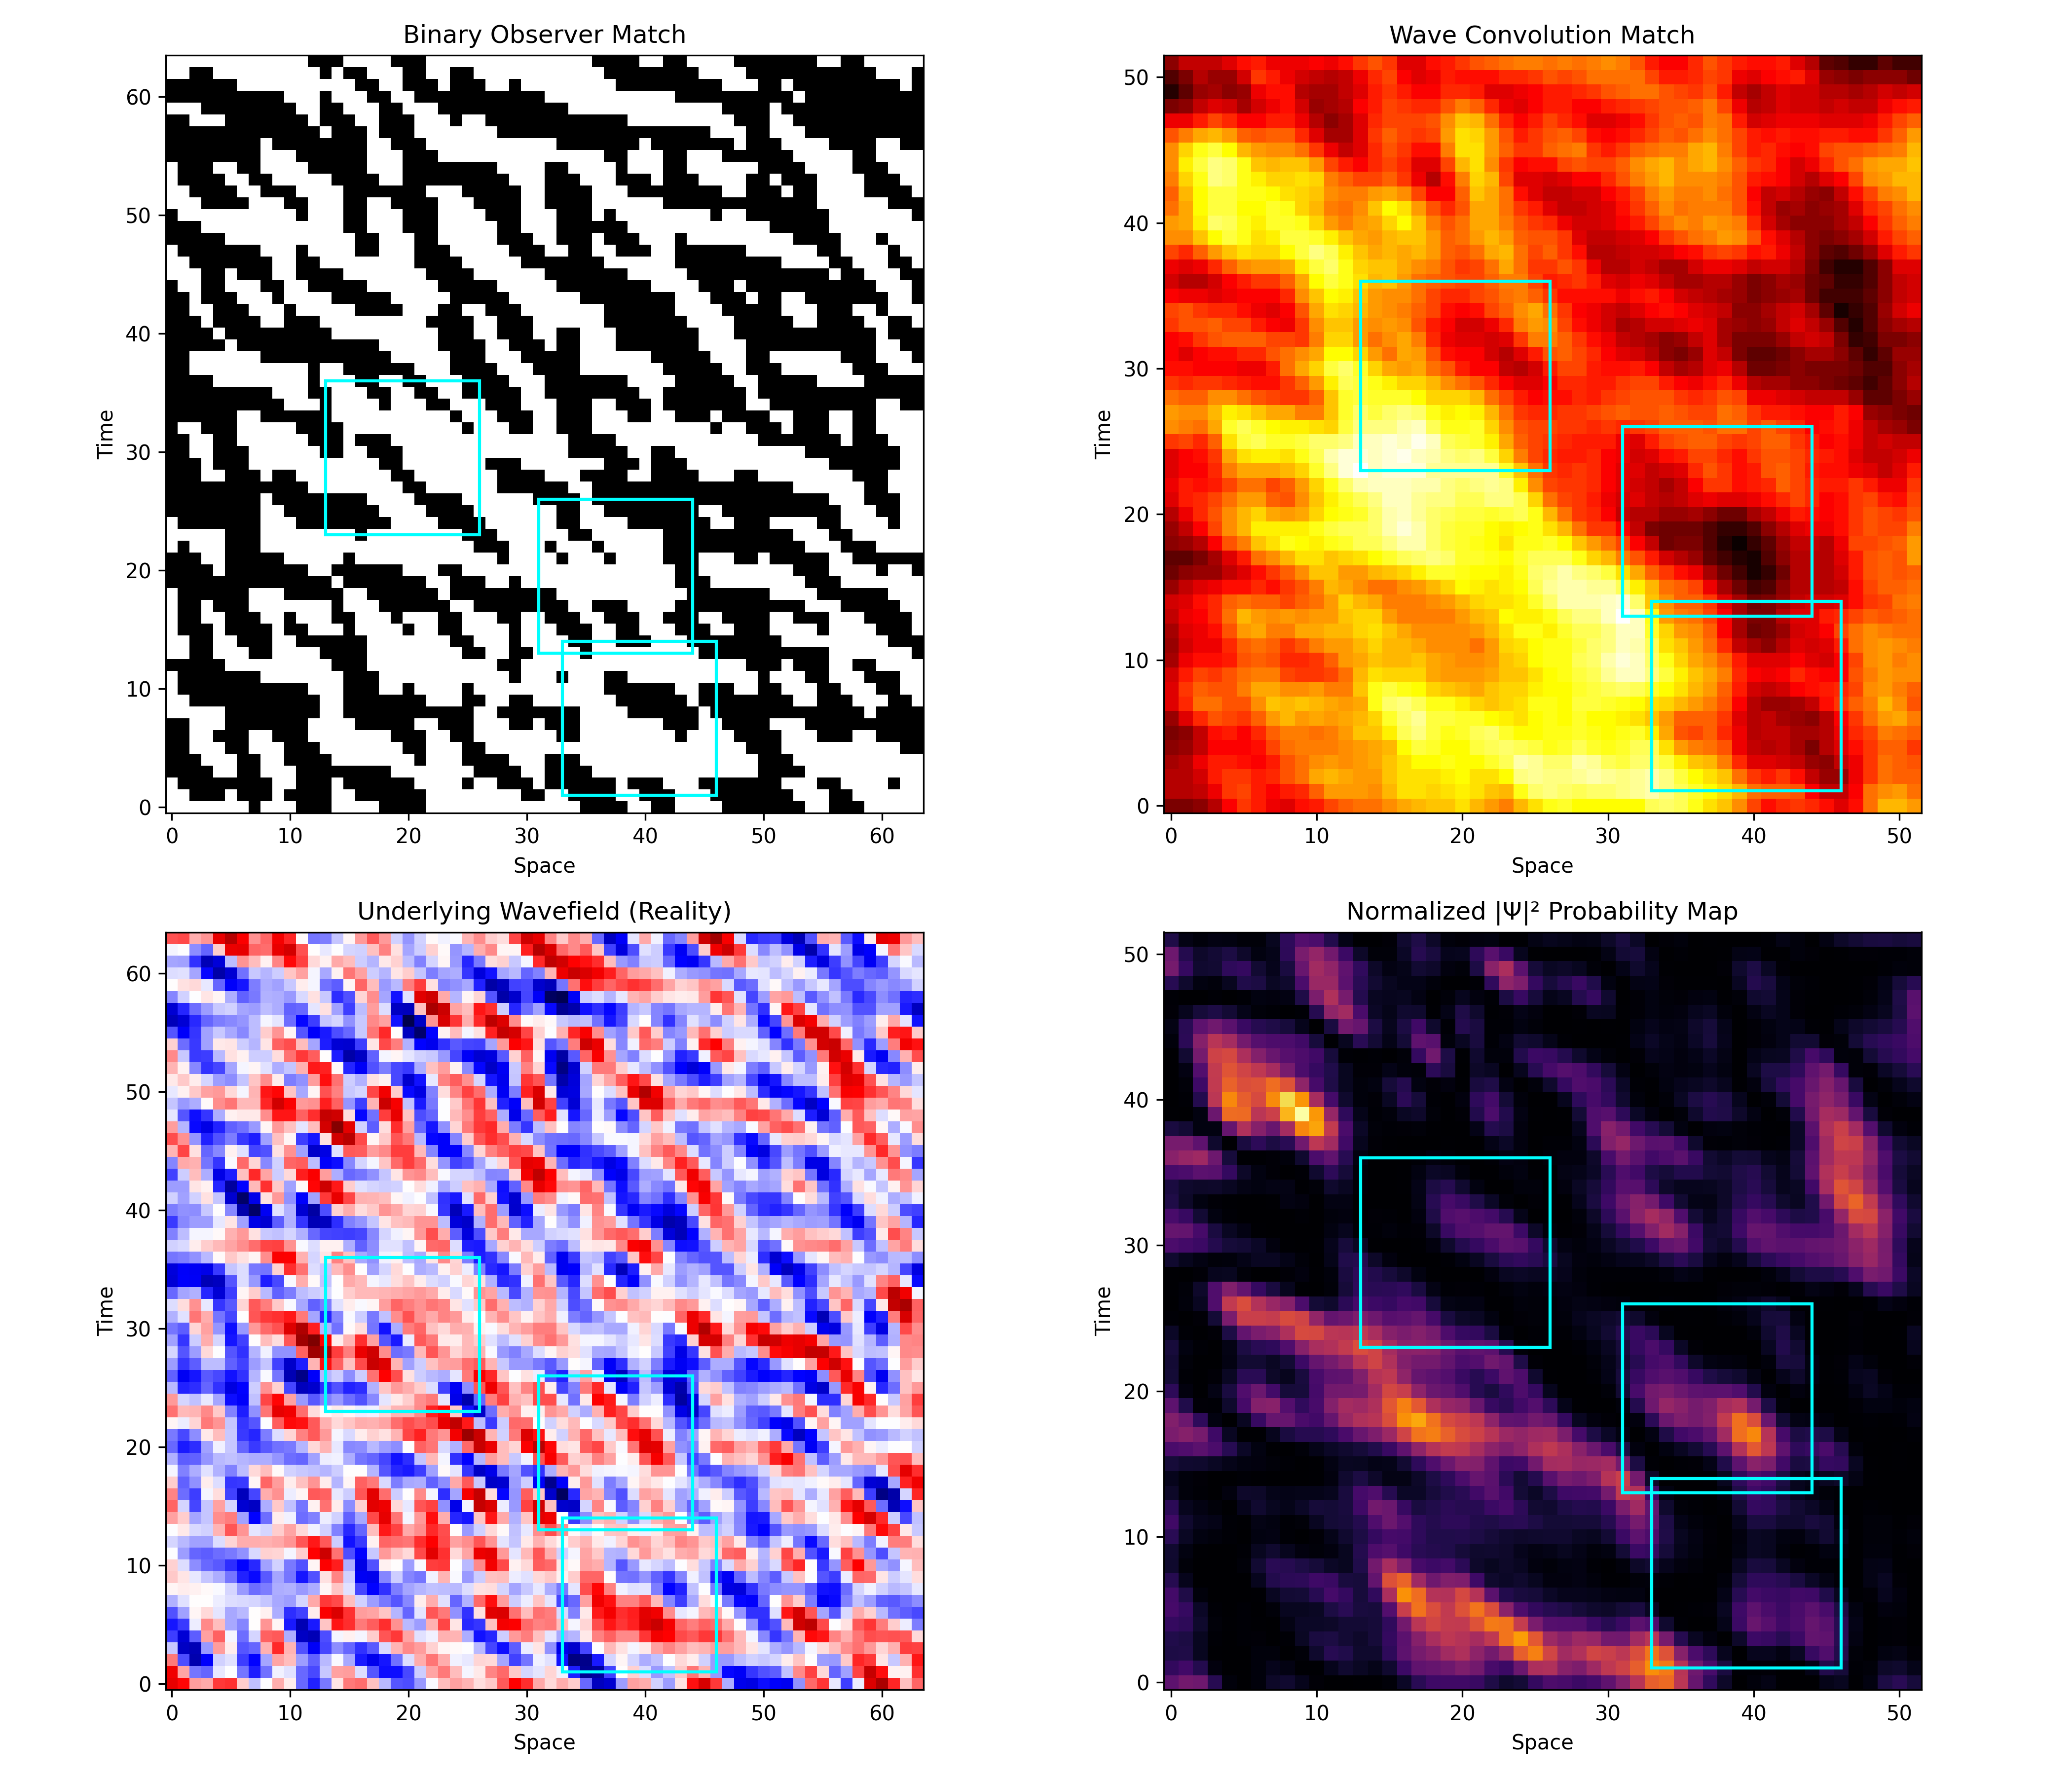
\includegraphics[width=1.0\textwidth]{figures/observer_wave_evolution.png}
    \caption{Four heatmaps visualizing observer wave evolution in spacetime.}
    \label{fig:observer_wave_evolution}
\end{figure}

The \textit{past} consists of those regions where the observer has high similarity. The \textit{future} consists of regions with no shared subsets, but which the observer can anticipate via extrapolation of its wavefunction.

\begin{figure}[h!]
    \centering
    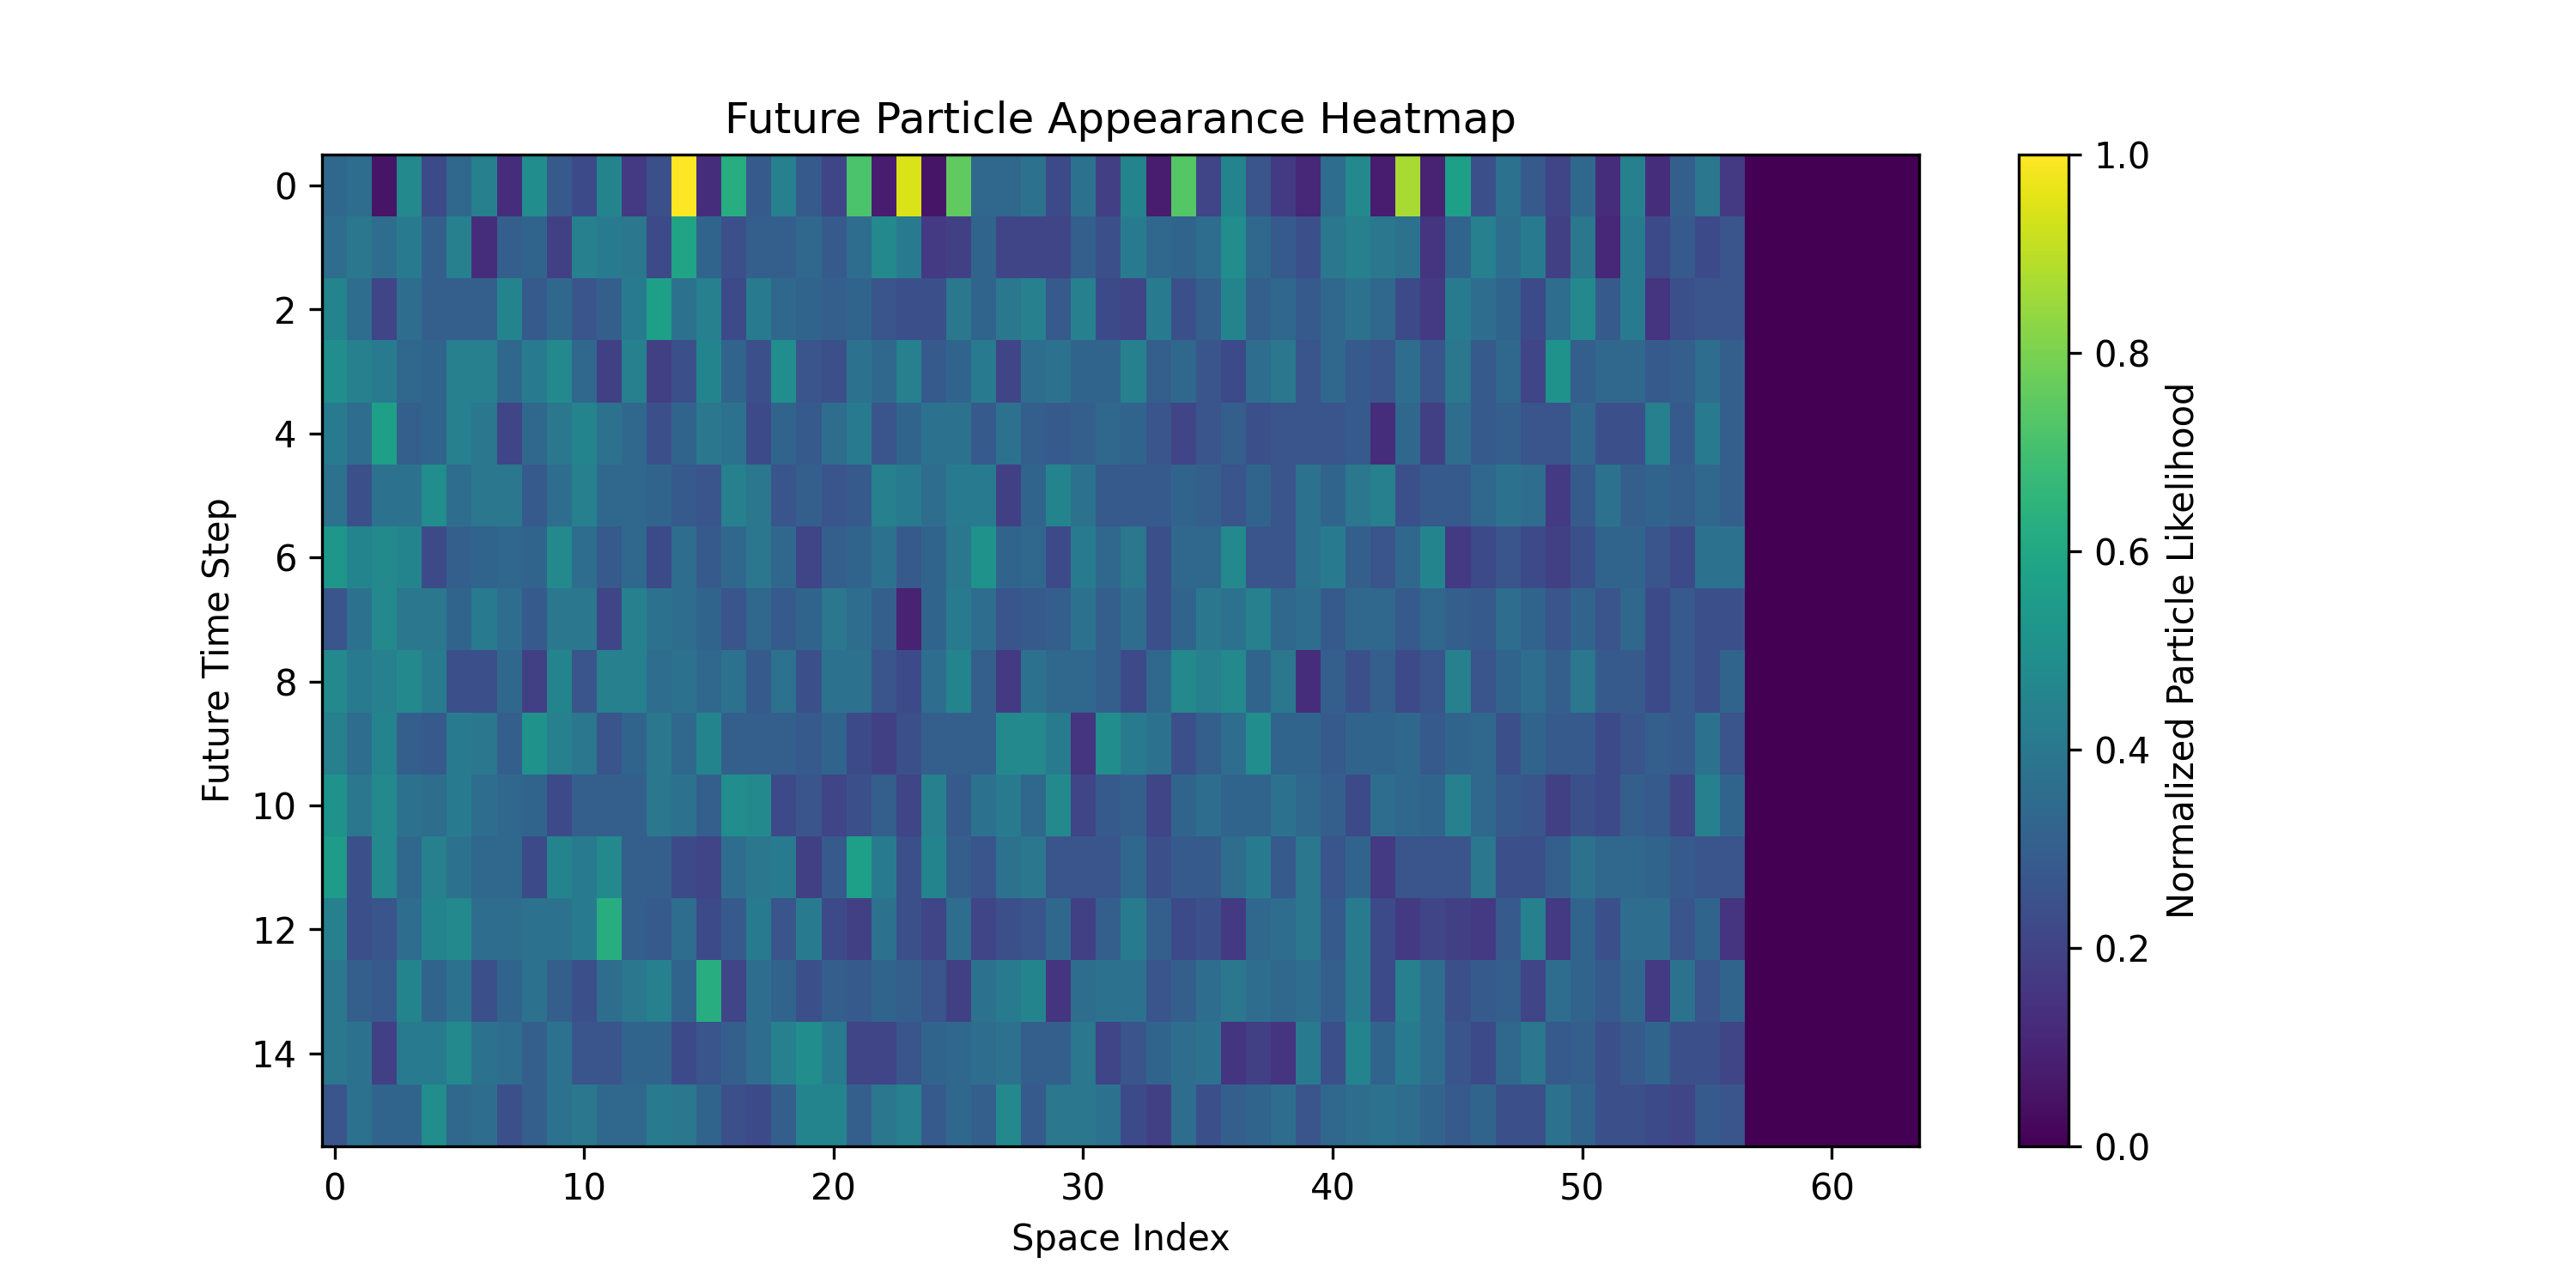
\includegraphics[width=1.0\textwidth]{figures/future_particle_heatmap.png}
    \caption{Heatmap visualizing likely future worlds. The density of particle trajectories illustrates where observers are most likely to find consistent continuations. The future is not a single path, but a distribution of possibilities shaped by the observer's current structure. Predictability fades rapidly with increasing distance from the present.}
    \label{fig:future_particle_heatmap}
\end{figure}

The program is available at:
\[
    \texttt{http://github.com/juhakm/simulations/paper2/simulation.py}
\]

\end{document}
